\documentclass[a4paper,
fontsize=11pt,
%headings=small,
oneside,
numbers=noperiodatend,
parskip=half-,
bibliography=totoc,
final
]{scrartcl}

\usepackage[babel]{csquotes}
\usepackage{synttree}
\usepackage{graphicx}
\setkeys{Gin}{width=.4\textwidth} %default pics size

\graphicspath{{./plots/}}
\usepackage[ngerman]{babel}
\usepackage[T1]{fontenc}
%\usepackage{amsmath}
\usepackage[utf8x]{inputenc}
\usepackage [hyphens]{url}
\usepackage{booktabs} 
\usepackage[left=2.4cm,right=2.4cm,top=2.3cm,bottom=2cm,includeheadfoot]{geometry}
\usepackage[labelformat=empty]{caption} % option 'labelformat=empty]' to surpress adding "Abbildung 1:" or "Figure 1" before each caption / use parameter '\captionsetup{labelformat=empty}' instead to change this for just one caption
\usepackage{eurosym}
\usepackage{multirow}
\usepackage[ngerman]{varioref}
\setcapindent{1em}
\renewcommand{\labelitemi}{--}
\usepackage{paralist}
\usepackage{pdfpages}
\usepackage{lscape}
\usepackage{float}
\usepackage{acronym}
\usepackage{eurosym}
\usepackage{longtable,lscape}
\usepackage{mathpazo}
\usepackage[normalem]{ulem} %emphasize weiterhin kursiv
\usepackage[flushmargin,ragged]{footmisc} % left align footnote
\usepackage{ccicons} 
\setcapindent{0pt} % no indentation in captions

%%%% fancy LIBREAS URL color 
\usepackage{xcolor}
\definecolor{libreas}{RGB}{112,0,0}

\usepackage{listings}

\urlstyle{same}  % don't use monospace font for urls

\usepackage[fleqn]{amsmath}

%adjust fontsize for part

\usepackage{sectsty}
\partfont{\large}

%Das BibTeX-Zeichen mit \BibTeX setzen:
\def\symbol#1{\char #1\relax}
\def\bsl{{\tt\symbol{'134}}}
\def\BibTeX{{\rm B\kern-.05em{\sc i\kern-.025em b}\kern-.08em
    T\kern-.1667em\lower.7ex\hbox{E}\kern-.125emX}}

\usepackage{fancyhdr}
\fancyhf{}
\pagestyle{fancyplain}
\fancyhead[R]{\thepage}

% make sure bookmarks are created eventough sections are not numbered!
% uncommend if sections are numbered (bookmarks created by default)
\makeatletter
\renewcommand\@seccntformat[1]{}
\makeatother

% typo setup
\clubpenalty = 10000
\widowpenalty = 10000
\displaywidowpenalty = 10000

\usepackage{hyperxmp}
\usepackage[colorlinks, linkcolor=black,citecolor=black, urlcolor=libreas,
breaklinks= true,bookmarks=true,bookmarksopen=true]{hyperref}
\usepackage{breakurl}

%meta
%meta

\fancyhead[L]{E. Corredera \& Valérie Andres\\ %author
LIBREAS. Library Ideas, 44 (2023). % journal, issue, volume.
\href{https://doi.org/10.18452/x}{\color{black}https://doi.org/10.18452/x}
{}} % doi 
\fancyhead[R]{\thepage} %page number
\fancyfoot[L] {\ccLogo \ccAttribution\ \href{https://creativecommons.org/licenses/by/4.0/}{\color{black}Creative Commons BY 4.0}}  %licence
\fancyfoot[R] {ISSN: 1860-7950}

\title{\LARGE{Back to Green. Das Projekt GOAL und das Potenzial von Grün Open Access}}% title
\author{Enrique Corredera \and Valérie Andres} % author

\setcounter{page}{1}

\hypersetup{%
      pdftitle={Back to Green. Das Projekt GOAL und das Potenzial von Grün Open Access},
     pdfauthor={Enrique Corredera, Valérie Andres},
      pdfcopyright={CC BY 4.0 International},
      pdfsubject={LIBREAS. Library Ideas, 44 (2023).},
      pdfkeywords={open access, Grüner Weg, Zweitveröffentlichung, Bibliothek, Service, Repositorien ; green road, self-archiving, library, repository, service},
      pdflicenseurl={https://creativecommons.org/licenses/by/4.0/},
      pdfurl={https://doi.org/},
      pdfdoi={10.18452/},
      pdflang={de},
      pdfmetalang={de}
     }



\date{}
\begin{document}

\maketitle
\thispagestyle{fancyplain} 

%abstracts
\begin{abstract}
\noindent
\textbf{Kurzfassung}: «GOAL -- Unlocking the Green Open Access
Potential» (\href{https://opengoal.ch/}{https://open goal.ch/}) ist die kollektive Bestrebung
einer Gruppe von wissenschaftlichen Bibliotheken zur Förderung des
bisher wenig beachteten Potentials von Grün Open Access in der Schweizer
Publikationslandschaft. 

Nicht oder nur marginal im Fokus der Nationalen
Open-Access-Strategie sind die Fachhochschulen und Pädagogischen
Hochschulen sowie kleine landessprachliche Verlage. Zunehmend seltener
anerkannt wird auch der Weg der Open-Access-Zweitveröffentlichung oder
«Grün Open Access». Es scheint, als ob sich der Ball bei der Umsetzung
von Open Access zunehmend im Besitz der «Read \& Publish» Verträge und
in der Förderung des Goldenen Weges befindet. 

Die «grüne Alternative»
führt ein wenig wahrgenommenes Schattendasein am Rande des Spielfeldes
und gilt als wenig attraktiv. Offenbar können auch die Argumente der
Nachhaltigkeit und der erhöhten Sichtbarkeit nicht genügend überzeugen.
Aus Sicht des Projektes GOAL eröffnet der Grüne Weg jedoch einen in der
Schweiz noch wenig genutzten Handlungsspielraum, der sich jenseits der
grossen Verlage oder bekannten Universitäten befindet und ein nicht zu
unterschätzendes Potential hat. Das ist der Moment, in dem wir das Auge
auf praxisorientierte Zeitschriften richten, welche von kleinen
Verlagen, Fachgesellschaften oder öffentlichen Institutionen in den
verschiedenen Landessprachen publiziert werden. 

Diese Zeitschriften
haben bisher noch wenig Beachtung erhalten, obwohl sie eine
entscheidende Rolle für Forschende an Fach- sowie Pädagogischen
Hochschulen spielen. Hier ist das Spielfeld noch wenig besetzt und Open
Access kann, unter Berücksichtigung der Ressourcen der Redaktionen und
Hochschulen, noch aufgebaut werden. In unserem Beitrag stellen wir das
Projekt vor, präsentieren die Ergebnisse von anderthalb Jahren Arbeit
und stellen diese zur Diskussion.

\begin{center}\rule{0.5\linewidth}{0.5pt}\end{center}

\noindent \textbf{Abstract}: \enquote{GOAL -- Unlocking the Green Open Access Potential}
(\href{https://opengoal.ch/}{https://opengoal. ch/}) is the collective effort of a group of
academic libraries to promote the hitherto little-noticed potential of
Green Open Access in the Swiss publishing landscape. 

Universities of
applied sciences and of teacher education as well as small publishers in
vernacular languages have until now been only marginally in the focus of
the Swiss National Open Access Strategy. Similarly, the option of
self-archiving or \enquote{Green Open Access} is hardly recognized as a
solution. \enquote{Read \& publish} agreements and the \enquote{Gold Open Access}
option seem to be the preferred and most promoted forms of implementing
Open Access. 

The \enquote{green alternative} lives thus a little-perceived
shadowy existence on the fringes of the field and is seen as having
little appeal. Apparently, the arguments of sustainability and increased
visibility are not convincing enough either. From the point of view of
the GOAL project, however, the \enquote{green path} opens up a scope for
action that is still little used in Switzerland, which lies beyond the
big publishing houses and well-known universities and has a potential
that should not be underestimated. It is time to turn our attention to
practice-oriented journals published by small publishers, professional
societies, or public institutions in the various national languages.

These journals have so far received little attention, even though they
play a crucial role for researchers at universities of applied sciences
as well as universities of teacher education. Here, the playing field is
still open and Open Access can be expanded, taking always into account
the resources of the editorial offices and universities. In our
contribution, we introduce the project, present the results of one and a
half years of work, and put them up for discussion.
\end{abstract}

%body
\hypertarget{einleitung-gruxfcn-in-einer-welt-von-gold}{%
\section{Einleitung: Grün in einer Welt von
Gold}\label{einleitung-gruxfcn-in-einer-welt-von-gold}}

Zu den ursprünglichen Zielen der Open Access-Bewegung gehörte die
strukturelle Transformation der akademischen Publikationslandschaft. Die
damals empfohlenen Strategien waren der Weg des Self-Archiving (also der
Veröffentlichung beziehungsweise parallelen Archivierung über gesicherte
Repositorien) und die Etablierung von alternativen Fachzeitschriften,
welche direkt Open Access erscheinen. Da jede Publikation Kosten mit
sich bringt, die abgedeckt werden müssen, sollten ebenso
Finanzierungsmodelle entwickelt werden, die das Publizieren in Open
Access ermöglichen.

Die Verlagsbranche stand Open Access zunächst skeptisch gegenüber und
versuchte, es zu konterkarieren. Nach kurzer Zeit allerdings baute sie
es aktiv nach ihren eigenen Interessen auf (Annemark, 2017). Dabei
wurden zwei von den drei Empfehlungen gefördert, die die Budapester
Deklaration\footnote{Budapest Open Access Initiative, siehe
  \url{https://www.budapestopenaccessinitiative.org/read/}}
hervorgehoben hatte, nämlich die Entwicklung neuer Finanzierungsmodelle
und die Kreation von alternativen Fachzeitschriften. So entstanden in
den letzten zwanzig Jahren viele neue Zeitschriften oder bereits
existierende wurden auf ein Open Access-Modell umgestellt. Diese
Kreationen und Transformationen kamen zusammen mit neuen
Finanzierungsmodellen; unser Vokabular erweiterte sich mit den
«Gold-Lösungen» und den «Article Processing Charges» (kurz APC genannt).

Anders ausgedrückt: Einundzwanzig Jahre später sieht die Welt
tatsächlich anders aus und eine Transformation hat stattgefunden. Open
Access ist keine Ausnahme mehr, sondern ein integraler Bestandteil der
Publikationslandschaft und der Hochschulpolitik. So visiert etwa die
Nationale Open-Access-Strategie der Schweiz für wissenschaftliche
Publikationen bis Ende 2024 100\,\% Open Access an.\footnote{Nationale
  Open-Access-Strategie der Schweiz, siehe
  \url{https://www.swissuniversities.ch/fileadmin/swissuniversities/Dokumente/Hochschulpolitik/Open_Access/Open_Access__strategy_final_DE.pdf}}

Diese neue Welt ist jedoch keineswegs befriedigend. Die Kosten für die
Bibliotheken sind nicht geringer geworden, da die Lösungen vor allem den
Interessen der großen Verlage dienen. Sowohl Publizierende als auch
Bibliotheken müssen die geeigneten Publikationswege zwischen
unterschiedlichen Fördervorgaben und einem wenig überblickbaren Angebot
an Open Access-Optionen finden, wobei die Publikationskosten für Gold in
teilweise unerreichbare Höhe gestiegen sind. Autor:innen und
Bibliotheken müssen eine neue Herausforderung -- die Kosteneinschätzung
-- meistern. Um alles noch komplexer zu machen, müssen sie auch die
Qualität der Open Access-Zeitschriften mit APC-Modellen einschätzen. Die
Grenzen zwischen mangelhafter Qualität und vorsätzlich betrügerischen
Geschäftsmodellen (Predatory Publishing) sind nicht auf den ersten Blick
ersichtlich (Dengler, 2023). Von Forschenden ist zu vernehmen, dass die
Zahl der aufdringlichen Werbemails von tatsächlichen oder vermeintlichen
Verlagen massiv zugenommen hat.

Mäßig befriedigend sind auch die transformativen «Read \& Publish»
Verträge (in Deutschland vor allem im Rahmen des DEAL-Projektes). Es hat
weder die erhoffte kostenneutrale Umstellung von Hybrid auf Gold
stattgefunden, noch können die Angebote ausreichend genutzt werden. Sei
dies, weil bestimmte Kontingente schon in der zweiten Jahreshälfte
aufgebraucht sind oder die Auswahl der Zeitschriften vorgegeben ist, so
dass besonders Forschende aus den technischen und
naturwissenschaftlichen Disziplinen davon profitieren.

Kurzum: Aktuell ist das Panorama von kostenintensiven Lösungen dominiert
(Gold und Hybrid OA). Die Open Access-Zweitveröffentlichung, die «grüne
Alternative», führt ein Schattendasein oder wird als unattraktiv
bezeichnet. Es kann daher nicht überraschen, dass im Jahr 2022 die
aktualisierte Version der Budapester Open Access Deklaration für eine
tiefgreifende Revidierung der Lage plädierte (Šimukovič,
2023).\footnote{The Budapest Open Access Initiative:20th Anniversary
  Recommendations siehe
  \url{https://access2perspectives.org/2022/03/the-budapest-open-access-initiative20th-anniversary-recommendations/}}

Wir vom Projekt GOAL denken, dass die Zeit gekommen ist, Open Access zu
überdenken und den aktuellen Entwicklungen anzupassen. Nach wie vor gibt
es Gründe, die für Open Access sprechen. Texte, die Open Access
veröffentlicht werden, erhalten mehr Resonanz als Texte, die in
„closed'' Zeitschriften publiziert werden (Wenaas, 2022). Auch die
Forderungen nach mehr Demokratie und Transparenz lassen sich nicht
einfach zur Seite schieben.

Zweitveröffentlichen, heutzutage als «Grün Open Access» bekannt, ist
eine nachhaltige Option, um Open Access weiter zu verbreiten, die wir
aus dem Schatten von Gold oder Hybrid heraus ins Rampenlicht bringen
möchten. Der grüne Weg hat ein noch weit unausgeschöpftes Potenzial, das
Bibliodiversität fördert und von dem Autor:innen, Bibliotheken, sowie
kleinere landessprachliche Fach- und Verbandszeitschriften
beziehungsweise Verlage, profitieren können. Unser Projekt GOAL --
Unlocking the Green Open Access Potential (\url{https://opengoal.ch/}),
läuft seit Januar 2022 und kann bereits von ersten Ergebnissen bei den
Bestrebungen zur Förderung von Grün Open Access berichten.

Die Berichterstattung der vergangenen 20 Monate soll das
Gestaltungspotential von interbibliothekarischer Kooperation
thematisieren und zeigen, wie die «grüne Lösung» eine Alternative sein
kann. Zum Einstieg werden wir den Ursprung und die Ziele des Projektes
GOAL darstellen. Darauffolgend fokussieren wir auf unsere bisherigen
Erfahrungen bei der angestrebten Kollaboration zwischen
Zeitschriftenredaktionen und Hochschulbibliotheken. Wir berichten, wie
wir uns als über die Schweiz und verschiedene Institutionen verteiltes
Team organisieren. Anhand eines Beispiels zeigen wir, welche ersten
Erfolge wir verbuchen können und wo unsere Ideale von der Wirklichkeit
abweichen.

\hypertarget{der-ursprung-von-oa-easi-zu-goal}{%
\section{Der Ursprung: Von OA-EASI zu
GOAL}\label{der-ursprung-von-oa-easi-zu-goal}}

GOAL basiert auf den Ergebnissen seines Vorgängerprojektes, «OA-EASI --
Open Access for Educational and Applied Sciences»\footnote{Projekt
  «OA-EASI -- Open Access for Educational and Applied Sciences» siehe
  \url{https://oa-easi.ch/das-projekt/}}, welches ebenfalls von
swissuniversities gefördert wurde und das Publikationsverhalten von
Angehörigen an Schweizer Fachhochschulen und Pädagogischen Hochschulen
untersuchte. Dabei wurde anhand einer Datenanalyse aus den betreffenden
Hochschulrepositorien festgestellt, dass im Gegensatz zu den
Universitäten häufig in kleineren landessprachlichen Fach- und
Verbandszeitschriften publiziert wird. Ausserdem wurden mit einer
kleinen Auswahl an (zahlenmässig) besonders relevanten Zeitschriften
Expert:inneninterviews durchgeführt, um die Haltung der Redaktionen zu
Open Access zu erfragen. Die Reaktionen waren mehrheitlich positiv,
jedoch zeigte sich, dass eine Umstellung auf Open Access nur unter
gewissen Bedingungen möglich ist. Die technisch und personell
limitierten Ressourcen verunmöglichen eine komplette Umwandlung der
Zeitschriften zu Gold oder Diamond Open Access (Rosenkranz et al.,
2022). Ebenso zeigen sich grössere Hürden aufgrund der sehr diversen und
komplexen Finanzierungsmodelle dieser Zeitschriften. Da viele jedoch
bereits niederschwellig zugänglich sind und einer Weiterverwendung nicht
grundsätzlich abgeneigt, zeigte sich hier das Potential des grünen
Weges. Diese Ergebnisse von OA-EASI wurden genutzt, um GOAL als Projekt
zu entwickeln.

\hypertarget{das-goal-projekt-unlocking-green-open-access-in-switzerland}{%
\section{Das GOAL-Projekt: Unlocking Green Open Access in
Switzerland}\label{das-goal-projekt-unlocking-green-open-access-in-switzerland}}

Das GOAL-Projekt, mit einer Laufzeit von drei Jahren (2022--2024,
gefördert von swissuniversities und angesiedelt an der Bibliothek der
ZHAW, Zürcher Hochschule für Angewandte Wissenschaften), ist die
kollektive Bestrebung einer Gruppe Schweizer Hochschulbibliotheken, die
über den grünen Weg die Kooperation mit kleineren Verlagen sowie
öffentlichen oder halböffentlichen Institutionen, die ergänzend zu ihrem
eigentlichen Auftrag eine eigene Zeitschrift herausgeben, fördern
möchte. Unser Kernteam besteht aus Open-Access-Spezialist:innen von fünf
unterschiedlichen Bibliotheken an Fachhochschulen und Pädagogischen
Hochschulen. Zu diesen gehören: ZHAW -- Zürcher Hochschule für
Angewandte Wissenschaften, HSLU -- Hochschule Luzern, FHNW --
Fachhochschule Nordwestschweiz, ZHdK -- Zürcher Hochschule der Künste
und von der PH-Freiburg -- Pädagogische Hochschule Freiburg.

Im ergänzenden Sounding Board mit Beratungsfunktion sind zwölf weitere
Bibliotheken vertreten.\footnote{GOAL Sounding Board. siehe
  \url{https://opengoal.ch/team/sounding-board/}} Auf diese Weise bringt
GOAL nicht nur Bibliotheken und Redaktionen an einen Tisch, sondern es
stärkt auch landesweit die Zusammenarbeit zwischen Bibliotheken an
Fachhochschulen und Pädagogischen Hochschulen. Die Meetings mit dem
Sounding Board finden einmal pro Semester online statt. Sie dienen der
Berichterstattung über die aktuellen Arbeitspakete sowie der
Weiterentwicklung des gesamten Projektes. Ausserdem wird die Meinung der
Boardmitglieder zu konkreten Fragen und Herausforderungen abgeholt.

Wir verfolgen gleich mehrere miteinander verbundene Ziele: An erster
Stelle soll die Zweitveröffentlichung in Hochschulrepositorien dank
passender Policies der Zeitschriften gefördert werden, so dass die
Publikationen von Forschenden an Fachhochschulen und Pädagogischen
Hochschulen mehr Resonanz finden sowie das Open-Access-Volumen erhöht
wird. Zweitens sollen die betreffenden Zeitschriften beziehungsweise
Verlage für ihr Publikum weiterhin attraktiv bleiben, ohne dass sie ihre
Finanzierungsmodelle und die technischen Infrastrukturen radikal ändern
müssen. Drittens ist das Projekt bestrebt, eine kostengünstige und
nachhaltige Lösung für alle involvierten Parteien (Autor:innen,
Redaktionen, Bibliotheken und die Leserschaft) zu finden.

Um diese Vision des grünen Weges in die Wirklichkeit umzuwandeln, hat
sich das Team konkrete Ziele gestellt: Im Dialog mit den Verleger- und
Herausgeber:innen entwickeln wir multilinguale Green Open Access
Policies, die die Zeitschriften implementieren sollen. Die vereinbarten
Policies sind danach auf deren Websites zugänglich, ergänzend werden sie
entweder in einer öffentlich zugänglichen Datenbank auf der
Projektwebsite zur Verfügung stehen, oder, sofern die Zeitschrift die
Kriterien erfüllt, in die Datenbank Sherpa Romeo aufgenommen.\footnote{Sherpa
  Romeo, siehe https://v2.sherpa.ac.uk/romeo/} Besonders letzteres
erhöht ihre internationale Visibilität. Ein weiteres Ziel ist die
effizientere Gestaltung der Workflows zwischen Redaktionen und
Bibliotheken. Die möglichst umfängliche Selbstarchivierung der
Publikationen in den Repositorien soll durch die Definition von
manuellen oder halbautomatisierten Workflows vereinfacht werden. Zudem
dokumentieren wir unsere Erfahrungen und gewonnenen Kenntnisse. Damit
sollen beim Projektende «Best Practices» der Implementierung von Open
Access Policies entstehen, die auf der Projektwebsite zugänglich sind.

\hypertarget{von-der-idee-zur-praxis-ein-werkstattbericht-aus-anderthalb-jahren-goal}{%
\section{Von der Idee zur Praxis: Ein Werkstattbericht aus
anderthalb Jahren
GOAL}\label{von-der-idee-zur-praxis-ein-werkstattbericht-aus-anderthalb-jahren-goal}}

Die ersten Schritte von GOAL waren von organisatorischen Fragen geprägt
(teaminterne Kommunikation, Meetingstruktur, Gestaltung des
kollaborativen Arbeitens). In der ersten Projektphase sind vor allem
eine Projektwebsite, ein erkennbares Logo und eine Zenodo-Community
entstanden. Zudem haben wir aktiv an verschiedenen grösseren
Veranstaltungen -- wie den Open-Access-Tagen 2022 in Bern und 2023 in
Berlin -- teilgenommen.\footnote{Zenodo Community für
  Projektpublikationen, siehe
  \url{https://zenodo.org/communities/goal/?page=1&size=20}

  Poster Open-Access-Tage 2022: Wie das GOAL-Projekt nachhaltige
  Kollaborationen zwischen Menschen, Maschinen und Strukturen fördert,
  siehe \url{https://doi.org/10.5281/zenodo.7038764}

  Vortrag Open-Access-Tage 2023: Gemeinsam den Grünen Weg gehen:
  Werkstattbericht des Projekts GOAL, siehe
  \url{https://doi.org/10.5281/zenodo.8389619}} Ausserdem wurden die
Daten der Publikationsanalyse über das Publikationsverhalten von
Angehörigen an Schweizer Fachhochschulen und Pädagogischen Hochschulen
aktualisiert.\footnote{«Bericht der Publikationsanalyse im Projekt
  GOAL», siehe \url{https://doi.org/10.5281/zenodo.7086670}} Des
Weiteren ist die geplante Datenbank im Aufbau und die ersten Ergebnisse
der Verhandlungen sind auf unserer Projektwebsite sichtbar.\footnote{Liste
  «Journals with Green Open Access Policy», siehe
  \url{https://opengoal.ch/project-goal/results/}}

In der zweiten Projektphase gilt es, die Kluft zwischen Ideal und Praxis
zu überwinden -- im Fokus standen und stehen dabei die Verhandlungen mit
Zeitschriften über die Annahme und Umsetzung einer grünen
Open-Access-Politik. Als Orientierung dafür diente uns die anhand der
Publikationsanalyse erstellte Kartographierung der
Publikationslandschaft Schweiz. Aus ihr wird ersichtlich, in welchen
Zeitschriften besonders häufig publiziert wird, welche Institution sie
herausgibt oder wer zum Zielpublikum gehört.

Ein entscheidender Schritt bei den Verhandlungen ist die
Vorbereitungsarbeit. In dieser Phase werden die Charakteristika der
betreffenden Zeitschrift identifiziert. Anhand einer Online-Recherche,
bei der die Website der Zeitschrift im Zentrum steht, sammeln wir
Informationen zu folgenden Punkten:

\begin{itemize}
\item
  Unterscheidung wissenschaftliche oder praxisorientierte Zeitschrift,
\item
  Disziplin beziehungsweise Thematik,
\item
  Geschäftsmodell (Abonnement, Mitgliedschaft etc.),
\item
  Finanzielle Struktur (Verein, Hochschulinstitution,
  öffentliche/halböffentliche Institution, privates Unternehmen),
\item
  Unterscheidung digitale und/oder gedruckte Erscheinungsweise,
\item
  Vorhandensein DOI oder ISSN,
\item
  Anzahl der Ausgaben pro Jahr,
\item
  beteiligte Personen (Autor:innen, Redakteur:innen),
\item
  Ressourcen in den Redaktionen (Teilzeit, Vollzeit, Ehrenamt),
\item
  Unterscheidung Einsprachig- oder Mehrsprachigkeit,
\item
  Zielpublikum (Fachverbände, Wissenschaft, private Unternehmen),
\item
  Nähe zur Wissenschaftscommunity,
\item
  Existieren bereits Faktoren, die die Umsetzung von Open Access
  erleichtern? (Online-Lesezugang oder ähnliches)
\item
  Werden in den Publikationen Drittmaterialien verwendet, die bei der
  Wahl der Lizenz zu berücksichtigen sind?
\item
  Können wir auf bereits existierende Kontakte aus unserem Umfeld
  anknüpfen?
\end{itemize}

Die hier nicht abschliessend aufgelisteten Checkpunkte geben uns eine
Orientierung bei der Zielsetzung und helfen, bereits im Voraus
individuell angepasste Angebote auszuarbeiten.

In der massgeschneiderten Lösung müssen sowohl die einzelnen Elemente
der Policy als auch deren langfristige Umsetzung mitgedacht werden. Je
nach Entscheidungskompetenzen in den Redaktionen bedeutet bereits die
Erstellung und Verabschiedung einer Policy, dass weitere
Entscheidungsträger:innen einzubeziehen sind. Sofern die Policy als
separates Dokument erstellt wird, muss ein geeigneter Ort auf der
Website gefunden werden. Als Alternative kann eine verkürzte Version der
Richtlinien im Impressum oder den Autor:innenrichtlinien aufgeführt
werden.

\pagebreak
Folgende Punkte stellen aus Sicht des GOAL-Projektes ein ideales
Verhandlungsergebnis dar:

\begin{itemize}
\item
  Nutzungslizenz CC BY, Rechte an Drittmaterialien geklärt
\item
  Policy auf Website der Zeitschrift
\item
  Lizenz im PDF vermerkt
\item
  Journal auf Sherpa Romeo gelistet (erfüllt Kriterien)
\item
  publizierte Version als PDF an Autor:innen oder Bibliotheken
\end{itemize}

Trotz sorgfältiger Vorbereitung vor der ersten Kontaktaufnahme gibt es
immer eine Unbekannte zwischen idealem Ziel und tatsächlicher Umsetzung.
In der Praxis lassen sich unerwartete Fragen oder unbeachtete
Perspektiven seitens der Redaktionen nicht komplett vermeiden;
Anpassungen und Kompromisse sind nötig, um eine Policy zu vereinbaren.

Anhand einer Zeitschrift aus der Bundesverwaltung, einer öffentlichen
Institution, möchten wir unsere Herausforderungen und Learnings
beschreiben: Die Autor:innen der Zeitschrift stammen aus Verwaltung,
Versicherungen, Sozialen Institutionen sowie aus der Forschung. Seit
2021 erscheint die Zeitschrift ausschliesslich in elektronischer
Version. Die Artikel sind frei zugänglich, jedoch -- mit Verweis auf
integrierte Drittmaterialien -- ohne freie Lizenz. Es wurde entschieden,
kein separates Dokument für die Policy zu erstellen, sondern einen
Hinweis im Impressum auf der Website anzubringen (vergleiche Abbildung
1). Der zuvor schon existierende Hinweis zum Copyright sollte
beibehalten und um die Open Access Policy ergänzt werden. Von GOAL
wurden zwei denkbare Varianten für die Formulierung einer Policy zur
Verfügung gestellt, die danach im Team der Zeitschrift besprochen und an
gewissen Stellen angepasst wurden. Nachdem die Redaktion sich für die
endgültige Version entschieden hatte, wurde der deutsche Text von einem
Mitglied des GOAL-Teams ergänzend ins Französische übersetzt.

\begin{figure}[h!]
\centering
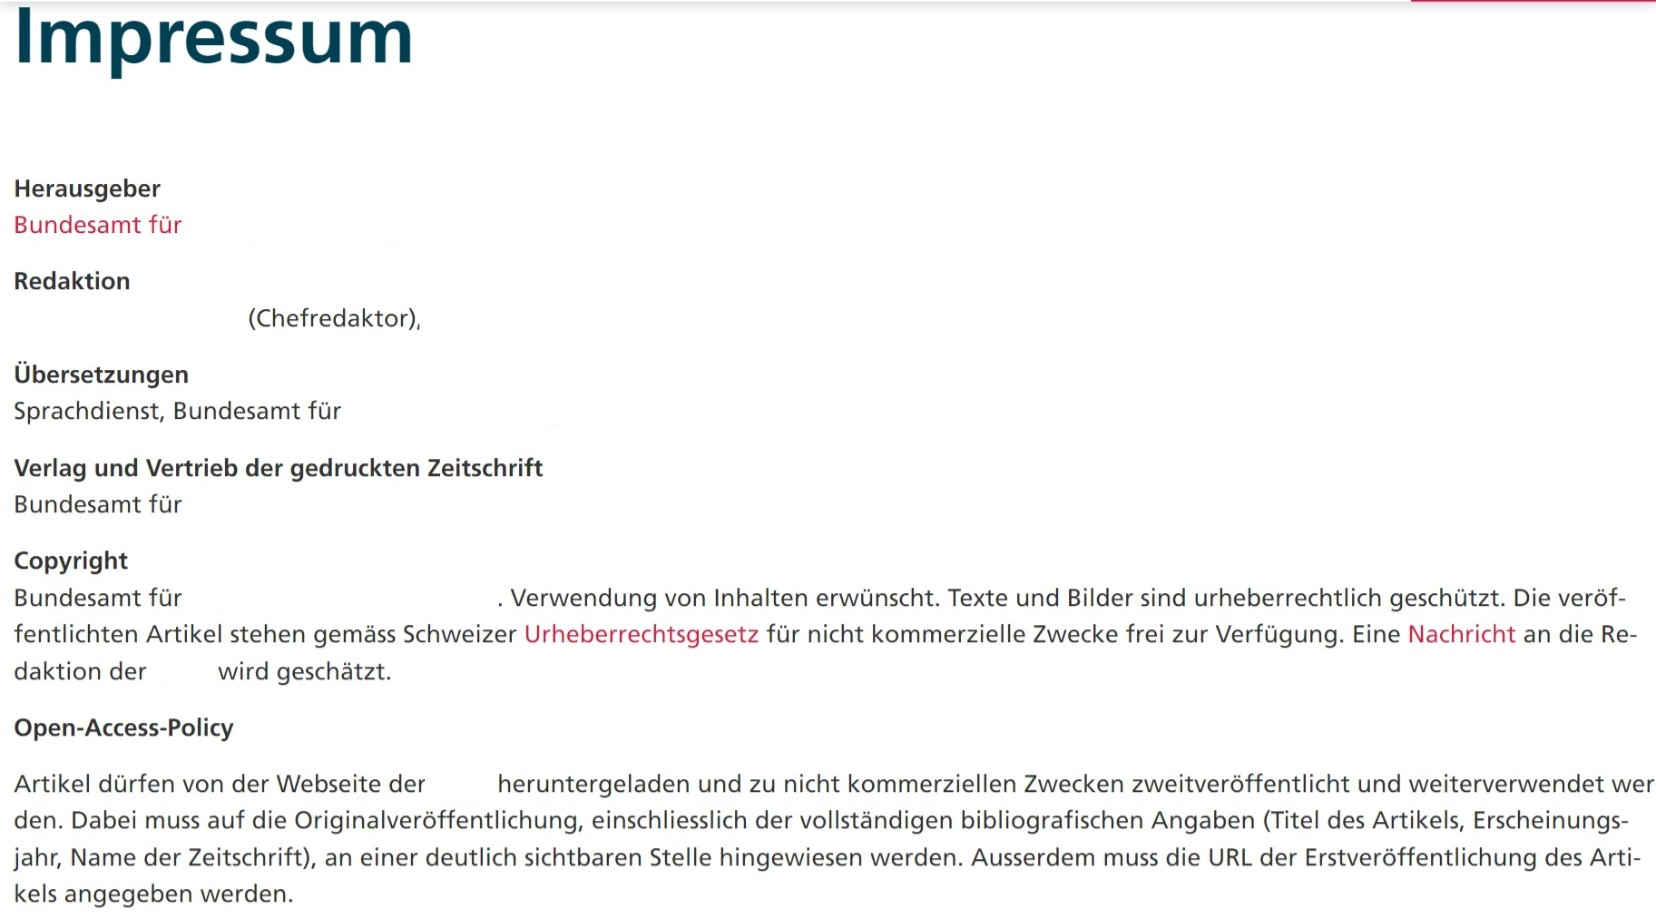
\includegraphics[width=0.9\textwidth]{img/andres_corredera_abb1.jpg}
\caption{Abbildung 1: Anweisungen zu Open Access beziehungsweise
Zweiveröffentlichungsrechten im Impressum der Zeitschrift.}
\end{figure}

Die Klärung von urheberrechtlichen Fragen erwies sich schnell als eine
der grössten Herausforderungen bei der Umsetzung von Green Open Access.
Die unendlichen Verbreitungs- und Wiederverwendungsmöglichkeiten in der
digitalen Welt bedeuten, dass die Rechte für Drittmaterialien, anders
als in den gedruckten Versionen, (aus)gehandelt werden müssen. Je
vielfältiger die Herkunft der integrierten Drittmaterialien, desto
aufwändiger sind die Rechteabklärungen. Daher ist entscheidend, wie hoch
der personelle Aufwand eingeschätzt wird und ob dieser in den
Redaktionen für jede Ausgabe geleistet werden kann. Die Alternativen zu
umfangreichen Abklärungen von integrierten Drittmaterialien sind
restriktivere Lizenzen, der explizite Ausschluss von Drittmaterialien
aus offeneren Lizenzen oder eine erhebliche Einschränkung der zur
Verfügung stehenden Quellen für die Autor:innen.

Bei dem oben genannten Beispiel war die Vergabe einer CC-Lizenz aufgrund
der integrierten Drittmaterialien nicht möglich: Die Inhalte richten
sich zwar explizit an eine möglichst breite Öffentlichkeit, jedoch soll
das Urheberrecht eingehalten und besonders eine kommerzielle Nachnutzung
ausgeschlossen werden. Lediglich die Weiterverbreitung soll eine
Erleichterung erfahren. Von dieser Lösung profitieren insbesondere die
Hochschulen und nicht profitorientierte Fachkreise, sowie
Privatpersonen. Faktisch wurde mit dieser Lösung ein gewisses Mass an
Offenheit geschaffen, die Erkenntnisse sind im Internet frei zugänglich
und sie können vom Zielpublikum im nichtkommerziellen Bereich geteilt
werden. Die Nachnutzung bleibt jedoch in einem geschlossenen Bereich.
Insgesamt ist die Policy eher schwer verständlich formuliert und sorgt
nicht für eine Abschaffung des rechtlichen Graubereichs des Status quo.
Für die Mitarbeitenden an den Hochschulen wird jedoch klar, dass dem
Upload der Artikel in den Repositorien nichts entgegensteht.

Bei dieser Zeitschrift zeigt sich auch exemplarisch der
Publikationsalltag und die damit verbundenen Hürden für die Umsetzung
von Zweitveröffentlichungen:

\begin{itemize}
\item
  OA-light: Erlaubnis zur Zweitveröffentlichung gemäss Urheberrecht auf
  dem Repositorium der Hochschule der Autor:innen. Vergabe einer
  CC-Lizenz eher selten.
\item
  Hinweis zu den Bedingungen der Zweitveröffentlichung ist im Impressum
  der Zeitschrift oder in den Autor:innenrichtlinien integriert. Keine
  ausformulierte Policy vorhanden.
\item
  PDF ist auf der Website zum Download oder über die Autor:innen
  verfügbar.
\item
  Die Redaktionen können keine strukturierten Metadaten liefern.
\item
  Die Artikel haben keinen DOI.
\item
  Die Zeitschrift hat keine ISSN.
\end{itemize}

Damit die Vorgaben in der Policy langfristig umgesetzt werden können,
muss darüber hinaus definiert werden, auf welchem Weg die Beiträge der
Forschenden in die Repositorien gelangen. Sind sie als PDF auf der
Webseite der Zeitschrift verfügbar oder wird den Autor:innen automatisch
ein Exemplar von der Redaktion zur Verfügung gestellt? Ist es möglich,
den Beitrag auf Artikelebene zu erhalten oder nur als ganze Ausgabe?
Inwiefern werden die Autor:innen in den Kommunikationsprozess mit
eingebunden, so dass sie weder zusätzlich belastet noch übergangen
werden?

Auch bei dieser Frage können sich unerwartete Hürden zeigen. In unserem
Beispiel werden die Texte direkt in ein Wordpress-«Gefäss» gegossen und
dann auf der Website publiziert. Somit verfügen weder Autor:innen noch
die Redaktion über ein PDF des publizierten Artikels. Ein Download als
PDF auf der Webseite ist technisch zwar möglich, optisch jedoch
unbefriedigend. Das Team der Zeitschrift hat auch diesen Punkt
diskutiert, jedoch aus Ressourcengründen entschieden, an diesem
Verfahren nichts zu ändern. Neben einer «finalen PDF-Version» fehlen
strukturierte Metadaten der Artikel, sowie ein DOI oder eine ISSN.

Der hier diskutierte Fall zeigt, dass bei der Erstellung einer Policy
nicht nur die Haltung gegenüber Open Access, sondern auch die
individuellen Ressourcen und technischen Voraussetzungen in den
Redaktionen berücksichtigt werden müssen. Auch das ist eine Aufgabe, die
sehr viel Zeit erfordert, weshalb das Team von GOAL aufgrund von
Informationen aus Erstgesprächen sowie eigenen Recherchen auf den
Webseiten der Zeitschriften massgeschneiderte Policies und
gegebenenfalls Workflows ausarbeitet. Es handelt sich dabei jedoch um
Vorschläge, die von den Redaktionen angenommen, verworfen oder
überarbeitet werden können. Die angebotene Lösung darf nicht als
Einmischung in die eigenen Angelegenheiten oder als Kritik wahrgenommen
werden.

Als Fazit des angeführten Beispiels lässt sich festhalten, dass wir es
bei dieser Zeitschrift mit einer sehr offenen und kooperativen Redaktion
zu tun hatten. Unsere Vorschläge wurden gewissenhaft geprüft und an die
eigenen Bedürfnisse angepasst. Die Anbindung der Redaktionsmitglieder an
die wissenschaftliche Community und die Kenntnisse zu Open Access waren
eher gering, die Offenheit für unsere Argumente hingegen gross. Auch von
Seiten des GOAL-Teams war zu diesem Zeitpunkt noch wenig Erfahrung
vorhanden. Alle diese Faktoren zeigen sich in dem zwar nicht perfekten,
jedoch sehr positiven Ergebnis und in der angenehmen Zusammenarbeit.

\hypertarget{fazit-gruxfcn-open-access-und-die-rolle-der-bibliotheken}{%
\section{Fazit: Grün Open Access und die Rolle der
Bibliotheken}\label{fazit-gruxfcn-open-access-und-die-rolle-der-bibliotheken}}

Wie das Beispiel zeigt, ist eine Förderung von Grün Open Access möglich
und nachhaltig. Die einzigen damit verbundenen Kosten für die
Zeitschriften betreffen die Zeit für Meetings mit GOAL, eventuelle
Anpassungen der Policy und die Klärung der Workflows bei deren
Implementierung. In der Regel handelt es sich dabei um einen Aufwand von
wenigen Stunden. Seitens der Bibliotheken ist die Lage etwas komplexer.
Die Expertise betreffend der Kenntnisse um Grün Open Access ist
mehrheitlich vorhanden oder kann in Detailfragen innerhalb des
bibliothekarischen Netzwerkes eingeholt werden. Da, wo das Wissen einer
Einzelperson nicht reicht, tauchen die Kolleg:innen als Unterstützung
auf. Die Zirkulation von Wissen zwischen den Bibliotheken kommt allen
zugute. Alle Bibliotheken investieren ein bisschen Zeit für den
gegenseitigen Informationsaustausch und die Verhandlungsvorbereitungen.
Jede neue vereinbarte Lösung (Policy und Workflows) bereichert den
gemeinsamen Erfahrungsschatz.

Bibliotheken prägen die Open-Access-Landschaft nicht nur durch ihre
Expertise, sie ermöglichen einen beträchtlichen Teil der Umsetzung auch
durch das Betreiben der Repositorien, durch weitere technische Lösungen
und ihre tägliche Arbeit als Dienstleistende für Publizierende und
Forschende. Anders ausgedrückt, sie sind fundamentale Akteure, wenn es
um die Infrastruktur geht, auf der Open Access basiert (Šimukovič, 2023:
281--318). Policies für Grün Open Access sind für Bibliotheken günstig
und nachhaltig, weil sie diese schon existierende Infrastruktur nutzen.
Da Bibliotheken auch eine langfristige Archivierungsaufgabe von
publizierten Materialien haben, müssen sie Repositorien unterhalten, auf
denen die Zweitveröffentlichungen erfolgen können.

Kurzum: Grün Open Access zeigt die entscheidende Rolle von Bibliotheken.
Durch Kooperation können Bibliotheken die Open-Access-Landschaft aktiv
prägen und mitgestalten. Im Fall des Projektes GOAL wurden bis dato
dreizehn Policies vereinbart und implementiert, sieben weitere wurden
vereinbart und müssen noch von den Zeitschriften veröffentlicht werden.

Dieses Gestaltungspotential muss aber im Einklang mit der alltäglichen
Realität kommen. Im Aufsatz haben wir geschildert, welche Vorarbeiten
nötig sind und wie die Abweichungen zwischen Ideal und Praxis aussehen.
Zusammenfassend haben wir drei grosse Hürden identifiziert, die unsere
Ergebnisse beeinflussen:

\begin{itemize}
\item
  Die Rechteklärung der verwendeten Drittmaterialien in den
  Publikationen erweist sich als grösste Hürde und Fass ohne Boden bei
  der Vergabe von CC-Lizenzen.
\item
  Die meist personell stark begrenzten Ressourcen in Redaktionen und
  Bibliotheken, welche für den Prozess mitgedacht werden müssen. Das
  betrifft sowohl die Erstellung der Policies als auch die
  Gewährleistung der zukünftigen Workflows.
\item
  Die Vorbehalte gegenüber «Offenheit» beziehungsweise Angst vor nicht
  absehbaren finanziellen oder rechtlichen Folgen beeinflusst die
  Ausformulierung der Policies.
\end{itemize}

\hypertarget{literaturliste}{%
\section{Literaturliste}\label{literaturliste}}

Annemark, M. (2017). Open Access och Big Business: hur Open Access blev
en del av de stora förlagen {[}Open Access and Big Business: How Open
Access Became a Part of Big Publishing{]}. Lund, Lund University
(Master thesis). Link online:
\url{https://lup.lub.lu.se/student-papers/search/publication/8923551}
{[}Accessed 10.10.2023{]}

Dengler, J. (2023). \enquote{Priorities in journal selection for
authors, reviewers, editors, librarians and science funders.}
\emph{Vegetation Classification and Survey,} 4: 1219--229. DOI:
\url{https://doi.org/10.3897/VCS.110296} {[}Accessed 10.10.2023{]}

Rosenkranz, S., Halbherr, V., Stricker, M., Reimer, N., Andres, V.,
Trautwein, C., Streitenberger, M. (2022). «Open Access an
Fachhochschulen, Hochschulen für angewandte Wissenschaften und
Pädagogischen Hochschulen -- Ergebnisse zweier Untersuchungen aus
Baden-Württemberg und der Schweiz» \emph{Informationspraxis}, 8:1
(Preprint),
\href{https://via.hypothes.is/https://informationspraxis.files.wordpress.com/2022/03/rosenkranz_etal_2022.pdf}{https://via.hypothes.is/https://informations praxis.files.wordpress.com/2022/03/rosenkranz\_etal\_2022.pdf}
{[}Accessed 10.10.2023{]}

Šimukovič, E. (2023). Of hopes, villains, and Trojan horses: Open Access
academic publishing and its battlefields. Wien, Universität Wien
(Doctoral thesis). DOI: \url{https://doi.org/10.21256/zhaw-28350}
{[}Accessed 10.10.2023{]}

Wenaas, L. (2022). Open Access: A Change in Academic Publishing with
Limited Reach? Oslo, University of Oslo (Doctoral thesis). Link online:
\url{http://hdl.handle.net/10852/97555} {[}Accessed 10.10.2023{]}

%autor
\begin{center}\rule{0.5\linewidth}{0.5pt}\end{center}

\textbf{Dr.~Enrique Corredera} ist promovierter Historiker im Rahmen
einer Cotutelle zwischen der Universität Konstanz (Deutschland) und der
Universidad Complutense de Madrid (Spanien). Zwischen 2017 und Juli 2021
war er Postdoktorand und Lehrbeauftragter an der Universität Bern. Seit
Januar 2021 arbeitet er an der Hochschulbibliothek der ZHAW (ROR ID:
\url{https://ror.org/05pmsvm27}), als Teil von Research \&
Infrastructure. Sein Schwerpunkt ist Open Science. Dr.~Corredera ist
seit Januar 2022 Projektkoordinator von GOAL. \\
ORCID ID: \url{https://orcid.org/0000-0002-4909-2415}

\textbf{Valérie Andres} hat Osteuropäische Geschichte und Russisch
studiert und sich auf Fotografie als historische Quelle spezialisiert.
Sie hat einen MAS in Information Science und ausgewiesene Erfahrung im
Bereich Bildrechte (Redakteurin im Pressebildbereich einer Bildagentur,
Spezialistin für Bilder im Staatsarchiv Aargau und ETH Bildarchiv). Seit
2016 ist sie an der Fachhochschule Nordwestschweiz tätig und hat dort
das Thema Open Access aufgebaut. Sie ist die Verantwortliche für Open
Access an der FHNW und Co-Präsidentin des Schweizer AKOA (Arbeitskreis
Open Access).

\end{document}